% when realtime?
% problem: efficiency, not open all socket for all resource
% only by demand! open/close socket room dynamically.

Realtime communication as mentioned in subsection \ref{subsection:concept-general-communication} are used for reactive data, which requires WebSocket for establishing persistent connections to enable the bi-directional communication between client and server.


All users are able to subscribe arbitrary course for new submission of a question as well as arbitrary question for updated order of answers, and server could also push realtime data to those users who has subscribed the resource with specific identifier. However, only two WebSocket services: \textit{/ws/courses} and \textit{/ws/questions} are defined as the entry points according to the definition in subsection \ref{subsection:websocket-definition-data-concept}. The approach how the server broadcast data precisely to the users who subscribe resources they require should be resolved.

A feasible solution is that the server maintains a list of user ids and resource ids subscribed by user. Afterwards, as a specific resource is updated, the server can get all users who has subscribed this resource from the maintained list using the resource's identifier.

\begin{figure}[!htbp]
  \centering
    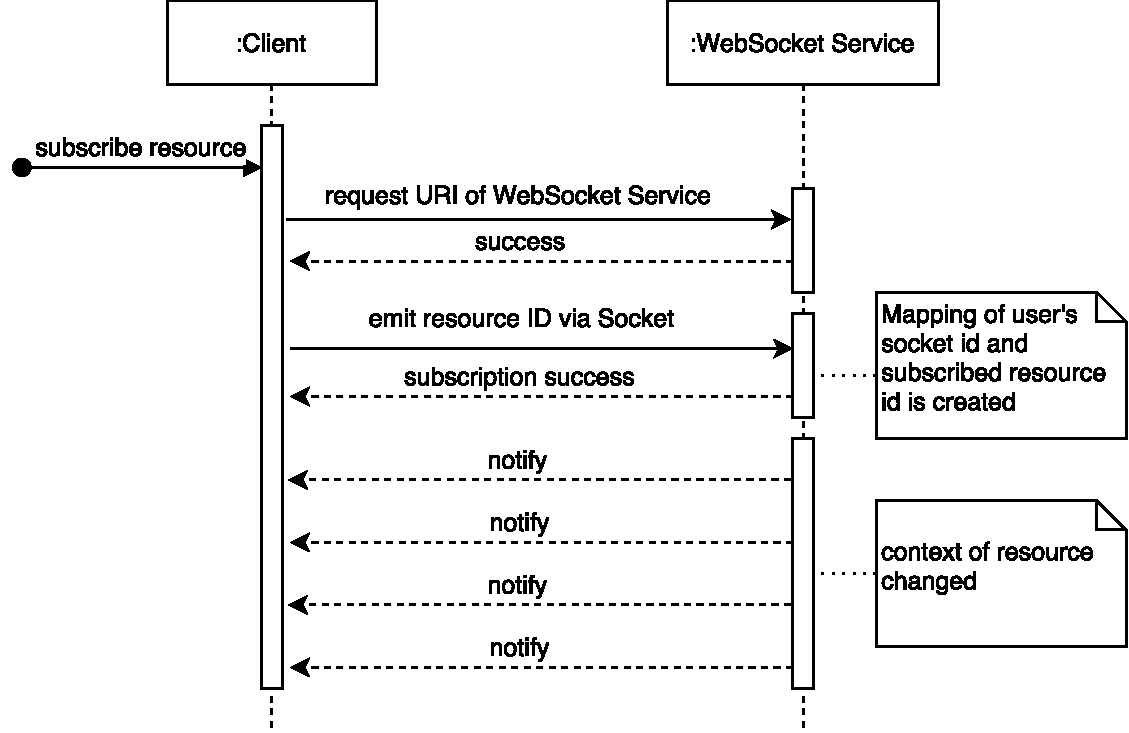
\includegraphics[width=1\textwidth]{Figures/concept-websocket-connection-sequence.pdf}
  \caption{Sequence diagram of establishing a WebSocket connection}
  \label{fig:websocket-connection-sequence-concept}
\end{figure}

%zhuangtaitu! status diagram!!! connected -> emit id to listen -> a list of mapping maintained by server.

Figure \ref{fig:websocket-connection-sequence-concept} represents the whole workflow of establishing the connection over WebSocket. In the first place, the server starts listening for requests over WebSocket protocol with specific URI. Then the user start a connection to server for subscribing the resource he requires. As soon as the connection is successfully established, the client will emit the resource id to the server side, and resource id from client will be mapped to the user id in a list maintained by the server.

After that, the server has the information of which user has subscribed which resource, and is able to emit realtime data precisely.